
% JuliaCon proceedings template
\documentclass{juliacon}
\setcounter{page}{1}

\begin{document}

% **************GENERATED FILE, DO NOT EDIT**************
\title{JuliaDB: addressing the two-language problem in analytical databases}

\author[1, 2]{Shashi Gowda}
\author[2]{Jeff Bezanson}
\author[2]{Josh Day}
\author[2]{Stefan Karpinski}
\author[2]{Viral B. Shah}
\author[3]{Pietro Vertechi}
\author[1]{Alan Edelman}
\affil[1]{Massachusetts Institute of Technology}
\affil[2]{Julia Computing Inc.}
\affil[3]{Champalimaud Centre for the Unknown}

\keywords{Julia, Databases, Analytics, Generic Programming}



\maketitle

\begin{abstract}


We present JuliaDB, a distributed database for analytical workloads
that is built solely in Julia, a high-level high-performance dynamic
language for numerical computing. JuliaDB is designed to allow seamless
use of user-defined Julia functions and data types. Julia's just-in-time compilation welds code from across Julia's package ecosystem as well as user code to generate efficient machine code allowing for high-performance data science in a coherent environment. We show example applications involving error analysis, mathematical optimization, online statistics, machine learning and linear algebra. 
\headingtable

\end{abstract}

\section{Introduction}


In~\cite{bezanson2017julia}, we describe the motivation behind Julia and how it was designed to address the two language problem: 
\begin{quote}
As long as the developers’ language is harder to
grasp than the users’ language, numerical computing will always be hindered. This is an essential part of the design philosophy of Julia: all basic functionality must be possible to implement in Julia—never force the programmer to resort to using C or Fortran.
\end{quote}

Modern data science workflows fall into two categories both of which show symptoms of the two language problem, the categories are:

\begin{enumerate}
\item Data is stored in traditional transaction-oriented databases (e.g. as Postgres and MySQL), queried with SQL, and analysed in high-level languages such as Python or R. This pairing suffers from two limitations: a) Most dialects of SQL, restrict custom data types and user defined functions, and b) The database server deals with on-disk data in a separate memory space from that of the analytics language making it an awkward combination for data science tasks.

\item Systems such as Pandas~\cite{mckinney-proc-scipy-2010} for Python and dplyr~\cite{dplyr} for R that provide a data storage and retrieval layer that is native to the host language. While they bring
the data into the memory space of the analytics language, they still
have some disadvantages: a) users must use vectorized database operations for performance since iterating over items in a loop can be expensive, and b) the need for vectorized operations to be 
implemented in C++, making it difficult to work with user defined data and functions. 
\end{enumerate}

Spark~\cite{spark} when used with Scala addresses many of the fundamental issues described above. However, Scala has been known to have performance concerns due to the design choices in the language~\cite{scalaslow}. In addition, users often use Spark through PySpark~\cite{pyspark} or SparkR~\cite{sparkr}, to gain the benefits of dynamically typed analytical languages. This brings us back to the two language problem.

We address the above mentioned two language problem in analytical databases with Julia~\cite{bezanson2017julia}. Its dynamic typing encourages exploratory and incremental programming. At the same time, users and database implementors have fine grained control over the memory layout of data. Struct types can be stored inline within arrays allowing efficient storage of user-defined
types. The just-in-time compiler can optimize data base operations and user defined functions as one system. Code from various packages written without the database in mind
can be used without performance penalties. In general, Julia finds the sweet-spot between dynamic
hassle-free languages such as Python and R helping the data scientist,
and efficient manually-memory-managed languages such as C or C++ helping
the database implementer greatly.


\section{Case study: manipulating measurements}
\label{sec:measurements}

Using the Measurements.jl ~\cite{giordano2016} package to represent physical measurements with some uncertainty. JuliaDB is unaware of the Measurement datatype, yet it can store measurements, read and write to disk and perform any database operation while using the math defined on the measurement type. In a two-language system, a performant implementation of the measurement datastructure must be done in a low-level language like C. For performant queries on databases containing measurements, one will have to implement an array of measurements datastructure in the low-level language as well. And tediously enumerate all possible array operations. But with JuliaDB and Julia, simply defining the measurement types and the primitive operations on Measurements is enough to achieve all the said features. Measurements can be stored efficiently in Julia arrays, operations such as `mean` and `sum` or broadcast on arrays of measurements fall out their existing generic implementations due to Julia's dynamic multiple-dispatch based JIT compiler.

Measurements.jl implements the ± operator
which represents an observation with some uncertainty associated
with it. Numeric operations on measuements propagate the
uncertainty as prescribed by linear error propagation theory:
For a function application $G(a,b,c...)$ where arguments are measurements $a=\overline{a} \pm \sigma_{a}, b=\overline{b} \pm \sigma_{b}, c=\overline{c} \pm \sigma_{c}$ the error of the output is found using the relationship:

$$
\begin{aligned}\sigma_{G}^{2}=&\left(\left.\frac{\partial G}{\partial a}\right|_{a=\overline{a}} \sigma_{a}\right)^{2}+\left(\left.\frac{\partial G}{\partial b}\right|_{b=\overline{b}} \sigma_{b}\right)^{2}+\left(\left.\frac{\partial G}{\partial c}\right|_{c=\overline{c}} \sigma_{c}\right)^{2}+\cdots \\
&+2\left(\frac{\partial G}{\partial a}\right)_{a=\overline{a}}\left(\frac{\partial G}{\partial b}\right)_{b=\overline{b}} \sigma_{a b}+2\left(\frac{\partial G}{\partial a}\right)_{a=\overline{a}}\left(\frac{\partial G}{\partial c}\right)_{c=\overline{c}} \sigma_{a c} \\ &+2\left(\frac{\partial G}{\partial b}\right)_{b=\overline{b}}\left(\frac{\partial G}{\partial c}\right)_{c=\overline{c}} \sigma_{b c}+\cdots \end{aligned}
$$\\

Where and $E[x]$ is the expected value of $x$.
Measurements.jl does not know about arrays, or JuliaDB, it just
defines how measurements get combined. Support for
measurements in the database in a non-julia analytical database
would involve having to write e.g. a mean function for an array
of measurements in C; in Julia, it emerges from dynamic
multiple dispatch, and compiles to C-like code.

Unlike a typical non-Julia analytical databases, without any
first class support for Measurements,
Pure-julia analytical database
We can store measurements directly in a JuliaDB table.

Perform groupby-mean without implementing the
mean function for an array of measurements in C.

Use OnlineStats for stats on measurements for lesser
allocation and parallelism.

\section{Designed of JuliaDB}

In the following subsection we describe the design of JuliaDB which empowers performance and interoperability.

\subsection{Memory layout}

The basic datastructure in JuliaDB is the table. A table can be constructed
from a Julia-native tuple or named tuple of column vectors. A table
acts as an iterator of rows. Rows are tuples or named tuples of items. 

Although the interface to a table is as a row iterator, the data is
stored column-wise for fast uniform access. The columns can be accessed
using the \texttt{columns} function (returns a named tuple of column
vectors). The rows can be accessed as an array of structs using the
\texttt{rows} function rows is a struct of arrays view into the columnar
storage, unlike table, \texttt{rows} returns a legitimate Julia array.
Listing 1 shows the workings of rows and columns.
\begin{lstlisting}[language=Julia]
julia> t = table((a=[1,2,3], b=[2,3,4]))
Table with 3 rows, 2 columns:
a  b

1  2
2  3
3  4
julia> columns(t)
(a = [1, 2, 3], b = [2, 3, 4])
julia> rows(t)
3-element StructArray{NamedTuple{(:a, :b),Tuple{Int64,Int64}},1,...}:
(a = 1, b = 2)
(a = 2, b = 3)
(a = 3, b = 4) 
\end{lstlisting}

Tables have a standard set of operations, below we almost just mention
them, we defer more detailed specification to the API documentation
{[}cite{]}. Mainly, they support \texttt{map}, \texttt{reduce}, \texttt{groupreduce}, \texttt{groupby} and \texttt{join} operations.

\subsection{Sort-based indexing}

We implement groupby and join by traversing tables in the key-order. We use counting sort wherever possible (e.g. integer columns, PooledArrays) to do a small amount of initial work on the order of $O(k \log k)$ where $k$ is the number of unique values and then acheive a sorted permutation in $O n$ time where $n$ is the number of rows. In most systems where the implementation is done in C++, the ordering routines are restricted to a handful of primitive data types. In our system any user defined data type with an \code{isless} method to compare two items can take part in the sorting.

\textbf{Indexing: }For speeding up table operations, you can tell
JuliaDB to keep the rows of a table sorted by some of its fields.
These fields are called primary key fields. The primary key fields
can be of any data type which has an \code{isless} method associated
with it to compare two values. This includes but is not limited to
numbers, strings, symbols, dates, time periods, currencies, quantities
of comparable physical units (e.g. inch, mm).

\subsection{Distributed compute}

A distributed table is a distributed analogue of the one described
above. It is stored as many tables across multiple Julia processes,
\code{columns} returns a tuple of \emph{distributed arrays} and
\code{rows} returns a distributed array of tuples! The distributed
arrays implementation has the usual array operations (map, reduce,
hcat, vcat) defined on it in a distributed manner. Constructing a
table with one or more distributed columns using the table constructor
results in a distributed table. We use the word ``table'' from now on to refer interchangeably to both types of tables, unless
noted otherwise.

Here we show benchmarks of JuliaDB against other popular data science
databases. Where appropriate, we turned off JuliaDB's distributed
features for fair comparison.

\subsection{CSV loading}

\begin{figure}[h]
\centering 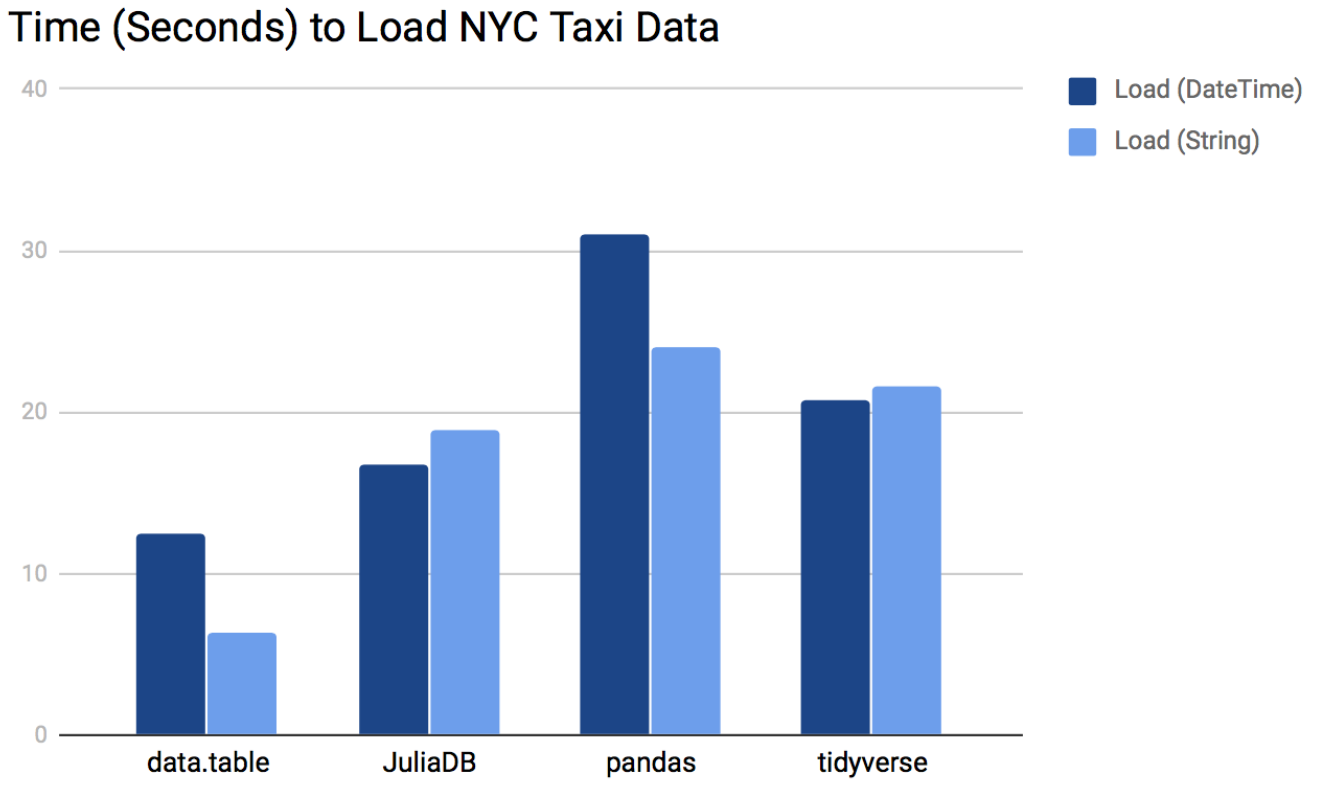
\includegraphics[width=5in]{image8.png} \caption{Performance comparison for loading 815MB from the NYC taxi dataset}
\label{fig:nyctaxiload} 
\end{figure}
Our test for loading data is an 815 MB CSV file from the NYC Taxi
\& Limousine Commission’s records on every yellow cab trip in January
of 2017. Figure~\ref{fig:nyctaxiload} compares loading times of
this data where the date-time fields are parsed as time objects or
simply as strings.

\subsection{Querying Data}

Our tests for querying involve three different tasks: 
\begin{enumerate}
\item Get the average “fare amount” by type of vendor. This is a standard
“group by” operation, calculating a statistic (mean) grouped by the
unique values in another column (type of vendor). 
\item Get the distribution of “number of passengers” by “day of week”. Here
we wish to count the number of trips where the number of passengers
is one, two, three, etc. grouped by the day of the week. 
\item Get the distribution of “number of passengers” by whether the weekday
number is even (Monday, Wednesday, Friday) or odd (Sunday, Tuesday,
Thursday, Saturday). Here we perform a similar “group by” operation
to the previous task, but use an arbitrary “group by” variable that
needs to depend on a user-defined function. 
\end{enumerate}
JuliaDB is the only platform that does not have a slowdown associated
with a UDF, with pandas taking the biggest hit (Figure~\ref{fig:nyctaxiquery}).

\begin{figure}[h]
\centering 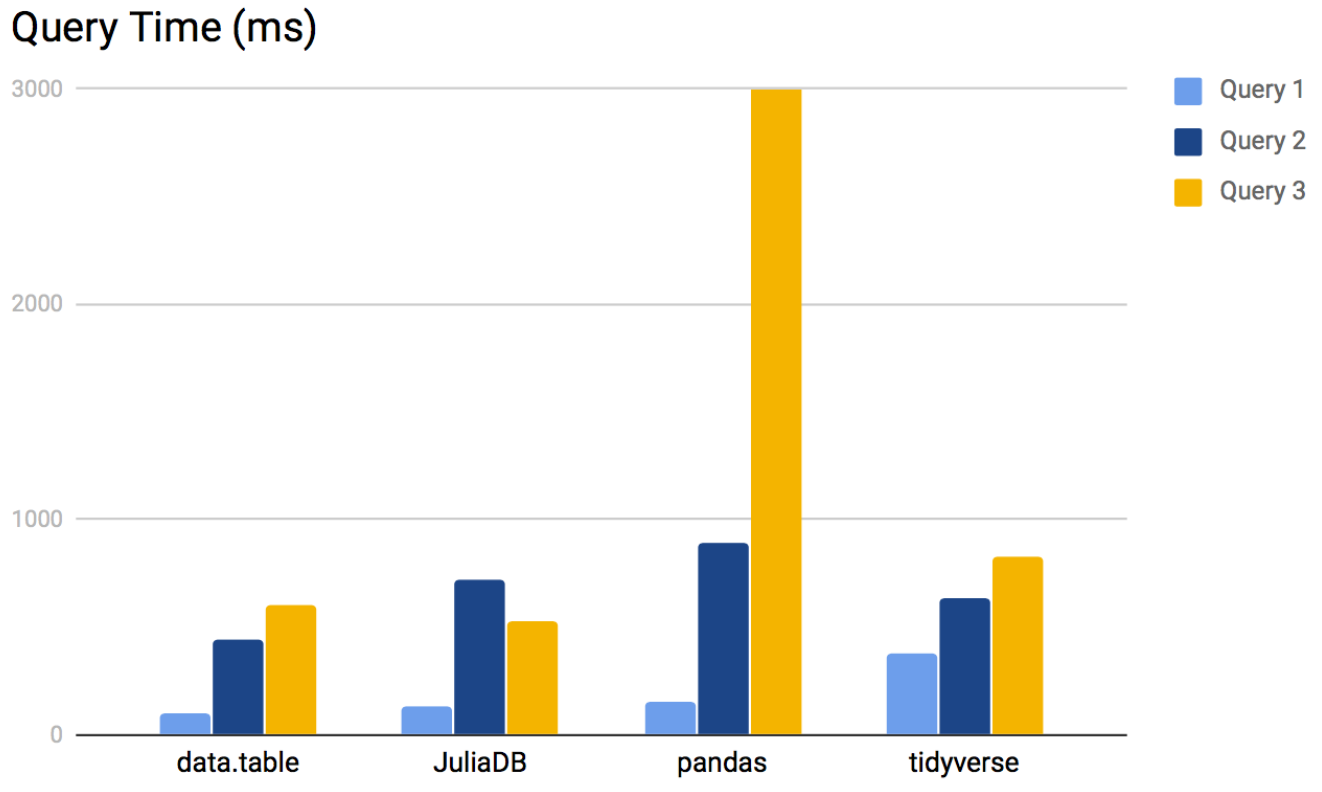
\includegraphics[width=5in]{image4.png} \caption{Query times for 3 different query types across various systems}
\label{fig:nyctaxiquery} 
\end{figure}

\section{Future directions}

1. AxisArrays
2. Query planning
3. More support for unstructured data

\section{Acknowledgements}

Tanmay Mohapatra, David Anthoff, Jacob Quinn


\section{Additional Document Style Options}
\label{sec:additional_doc}
%
The following additional style option is available with the \verb juliacon  class file:
\vskip 6pt
Please place any additional command definitions at the very start of
the \LaTeX{} file, before the \verb \begin{document} . For example, user-defined
\verb \def  and \verb \newcommand   commands that define macros for
technical expressions should be placed here. Other author-defined
macros should be kept to a minimum.
\vskip 6pt
Commands that differ from the standard \LaTeX{} interface, or that
are provided in addition to the standard interface, are explained in
this guide. This guide is not a substitute for the \LaTeX{} manual itself.
Authors planning to submit their papers in \LaTeX{} are advised to use
\verb \juliacon.cls  as early as possible in the creation of their files.

%
%
%
%
\begin{table*}[t]
\tabcolsep22pt
\tbl{If necessary, the tables can be extended both columns.}{
\begin{tabular}{|l|l|c|c|}\hline
Label & \multicolumn{1}{c|}{Description}
& Number of Users &
Number of Queries\\\hline
Test 1 & Training Data &
\smash{\raise-7pt\hbox{70}} & 104\\
\cline{1-2}\cline{4-4}
Test 2 & Testing Data I & & 105\\\hline
Test 3 & Testing Data II & 30 & 119\\\hline
& Total & 100 & 328\\\hline
\end{tabular}}
\label{tab:symbols}
\begin{tabnote}
This is an example of table footnote.
\end{tabnote}
\end{table*}
% \begin{figure*}[t]
% \centerline{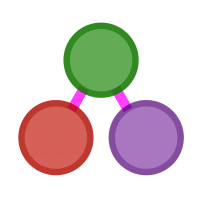
\includegraphics[width=11cm]{juliagraphs.png}}
% \caption{If necessary, the images can be extended both columns.}
%   \label{fig:sample_image}
% \end{figure*}

\section{Additional features}
\label{sec:additional_faci}
In addition to all the standard \LaTeX{} design elements, the \verb juliacon  class file includes the following features:
In general, once you have used the additional \verb juliacon.cls facilities
in your document, do not process it with a standard \LaTeX{} class
file.

\subsection{Titles, Author's Name, and Affiliation}
\label{subsub:title_auth}
The title of the article, author's name, and affiliation are used at the
beginning of the article (for the main title). These can be produced
using the following code:

\begin{verbatim}
\title{ This is an example of article title} }
\author{
   \large 1st Author \\[-3pt]
   \normalsize 1st author's affiliation  \\[-3pt]
    \normalsize 1st line of address \\[-3pt]
    \normalsize 2nd line of address \\[-3pt]
    \normalsize	1st author's email address \\[-3pt]
  \and
   \large 2nd Author \\[-3pt]
   \normalsize 2nd author's affiliation  \\[-3pt]
    \normalsize 1st line of address \\[-3pt]
    \normalsize 2nd line of address \\[-3pt]
    \normalsize	2nd author's email address \\[-3pt]
\and
   \large 3rd Author \\[-3pt]
   \normalsize 3rd author's affiliation  \\[-3pt]
    \normalsize 1st line of address \\[-3pt]
    \normalsize 2nd line of address \\[-3pt]
    \normalsize	3rd author's email address \\[-3pt]
}
\maketitle
\end{verbatim}

\subsection{Writing Julia code}

A special environment is already defined for Julia code,
built on top of \textit{listings} and \textit{jlcode}.

\begin{verbatim}
\begin{lstlisting}[language = Julia]
using Plots

x = -3.0:0.01:3.0
y = rand(length(x))
plot(x, y)
\end{lstlisting}
\end{verbatim}
\begin{lstlisting}[language = Julia]
using Plots

x = -3.0:0.01:3.0
y = rand(length(x))
plot(x, y)
\end{lstlisting}


\subsection{Abstracts, Key words, term etc...}
\label{subsub:abs_key_etc}

At the beginning of your article, the title should be generated
in the usual way using the \verb \maketitle  command. For genaral tem and keywords use
\verb \terms ,
\verb \keywords  commands respectively. The abstract should be enclosed
within an abstract environment, All these environment
can be produced using the following code:
\begin{verbatim}
\terms{Experimentation, Human Factors}

\keywords{Face animation, image-based modelling...}

\begin{abstract}
In this paper, we propose a new method for the
systematic determination of the model's base of
time varying delay system. This method based on
the construction of the classification data related
to the considered system. The number, the orders,
the time delay and the parameters of the local
models are generated automatically without any
knowledge about the full operating range of the
process. The parametric identification of the local
models is realized by a new recursive algorithm for
on line identification of systems with unknown time
delay. The proposed algorithm allows simultaneous
estimation of time delay and parameters of
discrete-time systems. The effectiveness of
the new method has been illustrated through
simulation.
\end{abstract}

\end{verbatim}

\section{Some guidelines}
\label{sec:some_guide}
The following notes may help you achieve the best effects with the
\verb juliacon  class file.

\subsection{Sections}
\label{subsub:sections}
\LaTeXe{}  provides four levels of section headings and they are all
defined in the \verb juliacon  class file:
\begin{itemize}
\item \verb \section   \item \verb \subsection  \item \verb \subsubsection  \item \verb \paragraph  \end{itemize}
Section headings are automatically converted to allcaps style.
\subsection{Lists}
\label{sec:lists}
%
The \verb juliacon   class file provides unnumbered lists using the
\verb unnumlist  environment for example,

\begin{unnumlist}
\item First unnumbered item which has no label and is indented from the
left margin.
\item Second unnumbered item.
\item Third unnumbered item.
\end{unnumlist}
The unnumbered list which has no label and is indented from the
left margin. was produced by:
\begin{verbatim}
\begin{unnumlist}
\item First unnumbered item...
\item Second unnumbered item...
\item Third unnumbered item...
\end{unnumlist}
\end{verbatim}

The \verb juliacon   class file also provides hyphen list using the
\verb itemize  environment for example,
\begin{itemize}
\item First unnumbered bulleted item which has no label and is indented
from the left margin.
\item Second unnumbered bulleted item.
\item Third unnumbered bulleted item which has no label and is indented
from the left margin.
\end{itemize}
was produced by:
\begin{verbatim}
\begin{itemize}
\item First item...
\item Second item...
\item Third item...
\end{itemize}
\end{verbatim}

Numbered list is also provided in acmtog class file using the
enumerate environment for example,
\begin{enumerate}
\item The attenuated and diluted stellar radiation.
\item Scattered radiation, and
\item Reradiation from other grains.
\end{enumerate}

was produced by:
\begin{verbatim}
\begin{enumerate}
\item The attenuated...
\item Scattered radiation, and...
\item Reradiation from other grains...
\end{enumerate}
\end{verbatim}
\subsection{Illustrations (or figures)}
\label{subsub:sec_Illus}
The \verb juliacon   class file will cope with most of the positioning of
your illustrations and you should not normally use the optional positional
qualifiers on the \verb figure   environment that would override
these decisions.
\vskip 6pt

%
\begin{figure}[t]
\centerline{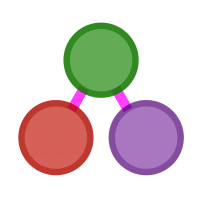
\includegraphics[width=4cm]{juliagraphs.png}}
\caption{This is example of the image in a column.}
	\label{fig:sample_figure}
\end{figure}

The figure \ref{fig:sample_figure} is taken from the JuliaGraphs
organization \footnote{https://github.com/JuliaGraphs}.

Figure captions should be \emph{below} the figure itself, therefore the
\verb \caption  command should appear after the figure or space left for
an illustration. For example, Figure 1 is produced using the following
commands:

\begin{verbatim}
\begin{figure}
\centerline{\includegraphics[width=20pc]{Graphics.eps}}
\caption{An example of the testing process for a
binary tree. The globa null hypothesis is tested
first at level $\alpha$ (a), and the level of
individual variables is reached last (d). Note
that individual hypotheses can be tested at
level $\alpha/4$ and not $\alpha/8$ as one might
expect at first.}
\label{sample-figure_2}
\end{figure}
\end{verbatim}
Figures can be resized using first and second argument of
\verb \includegraphics   command. First argument is used for modifying
figure height and the second argument is used for modifying
figure width respectively.
\vskip 6pt
Cross-referencing of figures, tables, and numbered, displayed
equations using the \verb \label  and \verb \ref   commands is encouraged.
For example, in referencing Figure 1 above, we used
\verb Figure~\ref{sample-figure}   \subsection{Tables}
\label{subsub:sec_Tab}
The \verb juliacon   class file will cope with most of the positioning of
your tables and you should not normally use the optional positional qualifiers on the table environment which would override these
decisions. Table captions should be at the top.
\begin{verbatim}
\begin{table}
\tbl{Tuning Set and Testing Set}{
\begin{tabular}{|l|l|c|c|}\hline
Label & \multicolumn{1}{c|}{Description}
& Number of Users &
Number of Queries\\\hline
Train70 & Training Data &
\smash{\raise-7pt\hbox{70}} & 104\\
\cline{1-2}\cline{4-4}
Test70 & Testing Data I & & 105\\\hline
Test30 & Testing Data II & 30 & 119\\\hline
& Total & 100 & 328\\\hline
\end{tabular}}
\end{table}\end{verbatim}

\begin{table}
\tbl{Tuning Set and Testing Set}{
\begin{tabular}{|l|l|c|c|}\hline
Label & \multicolumn{1}{c|}{Description}
& Number of Users &
Number of Queries\\\hline
Test 1 & Training Data &
\smash{\raise-7pt\hbox{70}} & 104\\
\cline{1-2}\cline{4-4}
Test 2 & Testing Data I & & 105\\\hline
Test 3 & Testing Data II & 30 & 119\\\hline
& Total & 100 & 328\\\hline
\end{tabular}}
\end{table}
\subsection{Landscaping Pages}
\label{subsub:landscaping_pages}
If a table is too wide to fit the standard measure, it may be turned,
with its caption, to 90 degrees. Landscape tables cannot be produced
directly using the \verb juliacon   class file because \TeX{} itself cannot
turn the page, and not all device drivers provide such a facility.
The following procedure can be used to produce such pages.
\vskip 6pt
Use the package \verb rotating   in your document and change the coding
from
\begin{verbatim}
\begin{table}...\end{table}
to
\begin{sidewaystable}...\end{sidewaystable}
and for figures
\begin{figure}...\end{figure}
to
\begin{sidewaysfigure}...\end{sidewaysfigure}
\end{verbatim}

environments in your document to turn your table on the appropriate
page of your document. For instance, the following code prints
a page with the running head, a message half way down and the
table number towards the bottom.
\begin{verbatim}
\begin{sidewaystable}
\tbl{Landscape table caption to go here.}{...}
\label{landtab}
\end{sidewaystable}
\end{verbatim}

\subsection{Double Column Figure and Tables}
\label{subsub:double_fig_tab}
For generating the output of figures and tables in double column
we can use the following coding:

\begin{enumerate}
\item For Figures:
\begin{verbatim}
\begin{figure*}...\end{figure*}
\end{verbatim}
\item For landscape figures:
\begin{verbatim}
\begin{sidewaysfigure*}...\end{sidewaysfigure*}
\end{verbatim}
\item For Tables:
\begin{verbatim}
\begin{table*}...\end{table*}
\end{verbatim}
\item For landscape tables:
\begin{verbatim}
\begin{sidewaystable*}...\end{sidewaystable*}
\end{verbatim}
\end{enumerate}

\subsection{Typesetting Mathematics}
\label{subsub:type_math}
The \verb juliacon class file will set displayed mathematics with center to
the column width, provided that you use the \LaTeXe{} standard of
open and closed square brackets as delimiters.
The equation
\[
\sum_{i=1}^p \lambda_i = (S)
\]

was typeset using the acmtog class file with the commands

\begin{verbatim}
\[
\sum_{i=1}^p \lambda_i = (S)
\]
\end{verbatim}

For display equations, cross-referencing is encouraged. For example,
\begin{verbatim}
\begin{equation}
(n-1)^{-1} \sum^n_{i=1} (X_i - \overline{X})^2.
\label{eq:samplevar}
\end{equation}
Equation~(\ref{eq:samplevar}) gives the formula for
sample variance.
\end{verbatim}
The following output is generated with the above coding:
\begin{equation}
(n-1)^{-1} \sum^n_{i=1} (X_i - \overline{X})^2.
\label{eq:samplevar}
\end{equation}
Equation~(\ref{eq:samplevar}) gives the formula for
sample variance.


\subsection{Enunciations}
\label{subsub:enunciation}
The \verb juliacon   class file generates the enunciations with the help of
the following commands:
\begin{verbatim}
\begin{theorem}...\end{theorem}
\begin{strategy}...\end{strategy}
\begin{property}...\end{property}
\begin{proposition}...\end{proposition}
\begin{lemma}...\end{lemma}
\begin{example}...\end{example}
\begin{proof}...\end{proof}
\begin{definition}...\end{definition}
\begin{algorithm}...\end{algorithm}
\begin{remark}...\end{remark}
\end{verbatim}
The above-mentioned coding can also include optional arguments
such as
\begin{verbatim}
\begin{theorem}[...]. Example for theorem:
\begin{theorem}[Generalized Poincare Conjecture]
Four score and seven ... created equal.
\end{theorem}
\end{verbatim}

\begin{theorem}[Generalized Poincare Conjecture]
Four score and seven years ago our fathers brought forth,
upon this continent, a new nation, conceived in Liberty,
 and dedicated to the proposition that all men are
created equal.
\end{theorem}


\subsection{Extract}
\label{subsub:extract}
Extract environment should be coded within
\begin{verbatim}
\begin{extract}..\end{extract}
\end{verbatim}

\subsection{Balancing column at last page}
\label{subsub:Balance}
For balancing the both column length at last page use :
\begin{verbatim}
\vadjust{\vfill\pagebreak}
\end{verbatim}

%\vadjust{\vfill\pagebreak}

at appropriate place in your \TeX{} file or in bibliography file.

\section{Handling references}
\label{subsub:references}
References are most easily (and correctly) generated using the
BIBTEX, which is easily invoked via
\begin{verbatim}
\bibliographystyle{juliacon}
\bibliography{ref}
\end{verbatim}
When submitting the document source (.tex) file to external
parties, the ref.bib file should be sent with it.
\cite{bezanson2017julia}

% **************GENERATED FILE, DO NOT EDIT**************

\bibliographystyle{juliacon}
\bibliography{ref.bib}


\end{document}

% Inspired by the International Journal of Computer Applications template
